% \chapter{Arquitectura y comandos b\'asicos}
\chapter{Arquitectura de grails}
Grails envuelve a muchas tecnolog\'ias relacionados con \textit{java}, abstrayendo su complejidad al proporcionarnos configuraciones predeterminadas que cubren los casos de uso m\'as comunes. Estas configuraciones pueden ahorrarnos d\'ias o semanas de trabajo debido a la integraci\'on con otras tecnolog\'ias.

Aqu\'i se presentan las tecnolog\'ias principales sobre las que se Grails est\'a montado:
%En este cap\'itulo se listan las tecnolog\'ias que usa grails y comandos b\'asicos para comenzar a usarlo. 

\begin{multicols}{2}
\begin{itemize}
  \item Hibernate
  \item Spring
  \item Sitemesh
  \item Tomcat
  \item H2
  \item Groovy
  \item Gant
  \item JEE
\end{itemize}
\end{multicols}

\begin{figure}[ht!]

    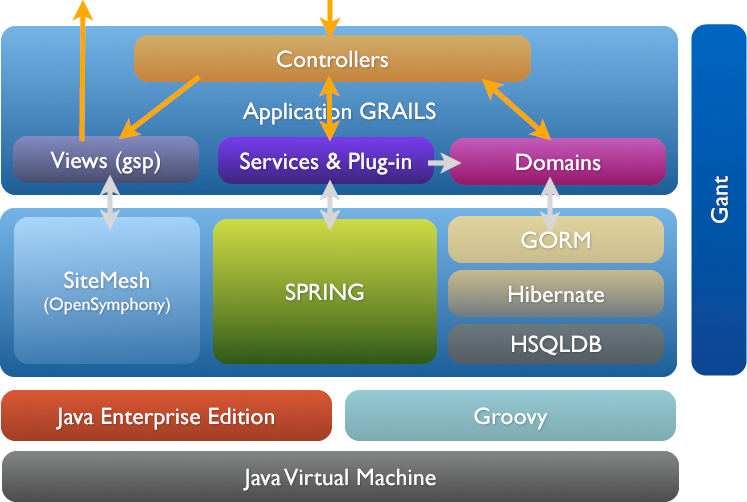
\includegraphics[width=100mm]{img/arch}
    \caption{Tecnolog\'ias que confirman la arquitectura de Grails}
    \label{arquitectura}
    

\end{figure}

